\documentclass[a4paper,11pt]{article}
\usepackage{amsfonts,amssymb,amsmath,amsthm,mathtools}
\usepackage{graphicx,xcolor,caption,subcaption,hyperref}

\RequirePackage[utf8]{inputenc}
\RequirePackage{cmap}
\RequirePackage[T2A]{fontenc}
\RequirePackage{csquotes}
\RequirePackage[russian]{babel}

\usepackage{tikz}
\usetikzlibrary{calc,patterns}
\makeatletter
\newcommand\currentcoordinate{\the\tikz@lastxsaved,\the\tikz@lastysaved}
\makeatother

\RequirePackage[margin=2.05cm,top=2.5cm,bottom=1.7cm]{geometry}
\linespread{1.08} \parskip=0.1in \parindent=0.4in

\usepackage{fancyhdr} \pagestyle{fancy}
\renewcommand{\headrulewidth}{0.22mm}
\headheight=16pt \headsep=6mm \footskip=6mm

\def\defaultstyle{
	\fancyhead[L]{{\sffamily Curriculum Vitae}}
	\fancyhead[R]{{\sffamily {\large Boris Zolotov,} {\footnotesize МКН СПбГУ}}}
	\fancyhead[C]{\ } \fancyfoot[C]{\thepage}
} \defaultstyle

\begin{document}

	\definecolor{tdefault}{RGB}{35,120,95}
	\def\tlineskip{0.545 cm}
	\def\tline#1#2{++(-0.6,-\tlineskip ) node[left]{#1} ++(0.6,0) node[right]{#2}}
	\def\tnline{++(0,-0.21cm)}

\def\tsection#1#2{
 \begin{center} \tikz{
     \fill[fill=tdefault] (-5,-0.13) rectangle (-0.6,0.13);
     \fill[fill=white] (0,-0.13) rectangle (11.8,0.13);
     \draw(0,0) node[right] {\LARGE\sffamily\textcolor{tdefault}{#1}}
	\tnline\tnline #2 ;
  } \end{center} \smallskip
}

\begin{center} \ \\ [0.4cm]
	{\Huge Boris Zolotov} \\ [0.35cm]
	{\textcolor{gray}{\it boris.a.zolotov@yandex.com \hspace{1.75cm} +7\,911\,764\,70\,83}}
\end{center} \vspace{0.2cm}

\tsection{Research Interests}{
	\tline{}{Theoretical computer science: algorithms, data structures,}
	\tline{}{computational geometry, automated proof systems}
}

\tsection{Education}{
		\tline{2021–present}{{\bfseries Ph.\,D. student,} St. Petersburg State University,}
		\tline{}{Department of Mathematics and Computer Sciences,}
		\tline{}{{\bfseries Researcher / Engineer,}}
		\tline{}{Euler International Mathematical Institute}
\tnline
		\tline{2019–2021}{{\bfseries MSc,} St. Petersburg State University,}
		\tline{}{Department of Mathematics and Computer Sciences,}
		\tline{}{„Advanced Mathematics“ MSc programme}
		\tline{\bf Title}{Algorithms for Dynamic Voronoi Diagrams}
		\tline{\bf Supervisor}{Candidate of Physics and Mathematics E. A. Arseneva}
		\tline{\bf Grade}{Excellent}
\tnline
	\tline{2015–2019}{{\bfseries BSc,} St. Petersburg State University,}
		\tline{}{Department of Mathematics and Computer Sciences,}
		\tline{}{„Mathematics“ BSc programme, bachelor's thesis:}
		\tline{\bf Title}{Algorithmic Aspects of Alexandrov's Uniqueness Theorem}
		\tline{\bf Supervisor}{Candidate of Physics and Mathematics E. A. Arseneva}
		\tline{\bf Grade}{Excellent}
}

\tsection{Student exchanges and internships}{
		\tline{10.2020 — 01.2021}{ULB, Brussels,\ \ Master en sciences}
		\tline{}{informatiques,\ \ Faculté des Sciences}
		\tline{}{(via competitive selection at SPBU)}
\tnline		\tline{\bf Courses}{{\tt Info-F409}\ \ Learning Dynamics}
		\tline{}{{\tt Info-F420}\ \ Computational Geometry}
		\tline{}{{\tt Info-F521}\ \ Graphs and Networks}
		\tline{}{{\tt Info-F413}\ \ Data Structures and Algorithms}
		\tline{}{{\tt Math-F513}\ \ Riemann Surfaces\vphantom{g}}
		\tline{}{{\tt Info-Y085}\ \ Functional Programming}
}

\tsection{Grants}{
	\tline{January 2020}{Russian Foundation for Basic Research (RFBR),}
	\tline{}{participant. Project title: Problems on the Border}
	\tline{}{of Combinatorics and Computational Geometry}
	\tnline\tline{September 2019}{2019 competition of the Foundation for the Advancement}
	\tline{}{of Theoretical Physics and Mathematics „BASIS“, participant}
}

\tsection{Teaching experience}{
\tnline \tline{2025–present}{{\bf “Advanced Data Structures”,}}
		\tline{}{III–IV year undergraduates, SPbU}
\tnline \tline{2023–present}{{\bf Seminars in Theoretical Computer Science,}}
		\tline{}{(algorithms, their implementation on C++, and related problems)}
		\tline{}{I–II semester undergraduates, SPbU}
\tnline \tline{09.–12.2022}{{\bf Seminars in Logic,}}
		\tline{}{V semester undergraduates, SPbU}
\tnline	\tline{2015–present}{Additional courses {\bf tutor},}
		\tline{}{Laboratory for Continuous Mathematical Education, St. Petersburg}
\tnline	\tline{2015–present}{{\bf Supervisor} of research projects for the youth,}
		\tline{}{Laboratory for Continuous Mathematical Education, St. Petersburg}
\tnline	\tline{2015–present}{Summer school courses {\bf tutor},}
		\tline{}{Laboratory for Continuous Mathematical Education, St. Petersburg}
\tnline	\tline{2018–2022}{Mathematics for Olympiads {\bf tutor,}}
		\tline{}{„Fractal“, St. Petersburg}
}

\tsection{Programming projects}{
\tnline \tline{Fall 2022}{{\it Profitability and accounting of goods,} soap factory “Aist”,}
                \tline{}{Python, SQL}
}

\tsection{Schools and workshops}{
\tnline \tline{January 2025}{{\bf Lecturer,} Winter Students' School on mathematics}
                \tline{}{and theoretical computer science, HSE, Moscow}
\tnline	\tline{June 2019}{Second Trans-Siberian Workshop on}
		\tline{}{Computational Geometry and Data Structures}
\tnline	\tline{November 2016}{Winter School on cubic plane curves, HSE, Moscow}
}

\newpage

\tsection{Community service}{
	\tline{August 2021}{{\bf Volunteer,} Conference of International}
	\tline{}{Mathematical Centers}
	\tnline
	\tline{August 2021}{{\bf Volunteer,} XX-th International}
	\tline{}{Congress on Mathematical Physics and}
	\tline{}{Young Researchers Symposium}
	\tnline
	\tline{April 2021}{{\bf Local organising committee} of EuroCG 2021}
	\tnline
	\tline{April 2018 — 2019}{{\bf Assistant \TeX -er} of Joint Projects of}
	\tline{}{PJSC Gazprom Neft and Chebyshev Laboratory}
	\tnline
	\tline{2016–present}{{\bf Supervisor of the project,}}
	\tline{}{„Mathematics Non-Stop“, Time for Science foundation}
	\tnline
	\tline{2016–2020}{{\bf Organising committee and jury,} Saint Petersburg}
	\tline{}{tournaments of young mathematicians}
	\tnline
	\tline{02.2018, 2019, 2020}{{\bf Jury,} Baltic Science And Engineering Fair}
}

\tsection{Preprints and Work in Progress}{
	\tline{2023–2024}{“Doubly-periodic string comparison” (“Affine LCS”)}
	\tline{}{(in {\it Combinatorial Pattern Matching,} with A.~Tiskin and N.~Gaevoy)}
\tnline \tline{2023–present}{“An Optimal Local Edit Distance Oracle”}
	\tline{}{(with A.~Tiskin and N.~Gaevoy)}
\tnline \tline{2025-present}{“Speeding up the BSP Convex Hull Algorithm”}
	\tline{}{(with A.~Tiskin and P.~Minkin)}
}

\tsection{Books and Brochures (in Russian)}{
		\tline{February 2019}{Б. А. Золотов, Д. Г. Штукенберг, И. А. Чистяков,}
		\tline{}{А. В. Семенов, И. С. Алексеев,}
		\tline{}{\it Сборник задач олимпиады «Математика НОН-СТОП»,}
		\tline{}{373 с., ISBN 978-5-906623-38-6}
\tnline	\tline{December 2019}{Б. А. Золотов, Д. Г. Штукенберг,}
		\tline{}{\it Математика НОН-СТОП—2019. Решения задач олимпиады,}
		\tline{}{72 с., ISBN 978-5-906623-47-8}
\tnline	\tline{December 2020}{Б. А. Золотов, Е. И. Тодоров, Д. Г. Штукенберг,}
		\tline{}{\it Математика НОН-СТОП—2020. Решения задач олимпиады,}
		\tline{}{80 с., ISBN 978-5-6045675-2-4}
} \newpage

\begin{center}
	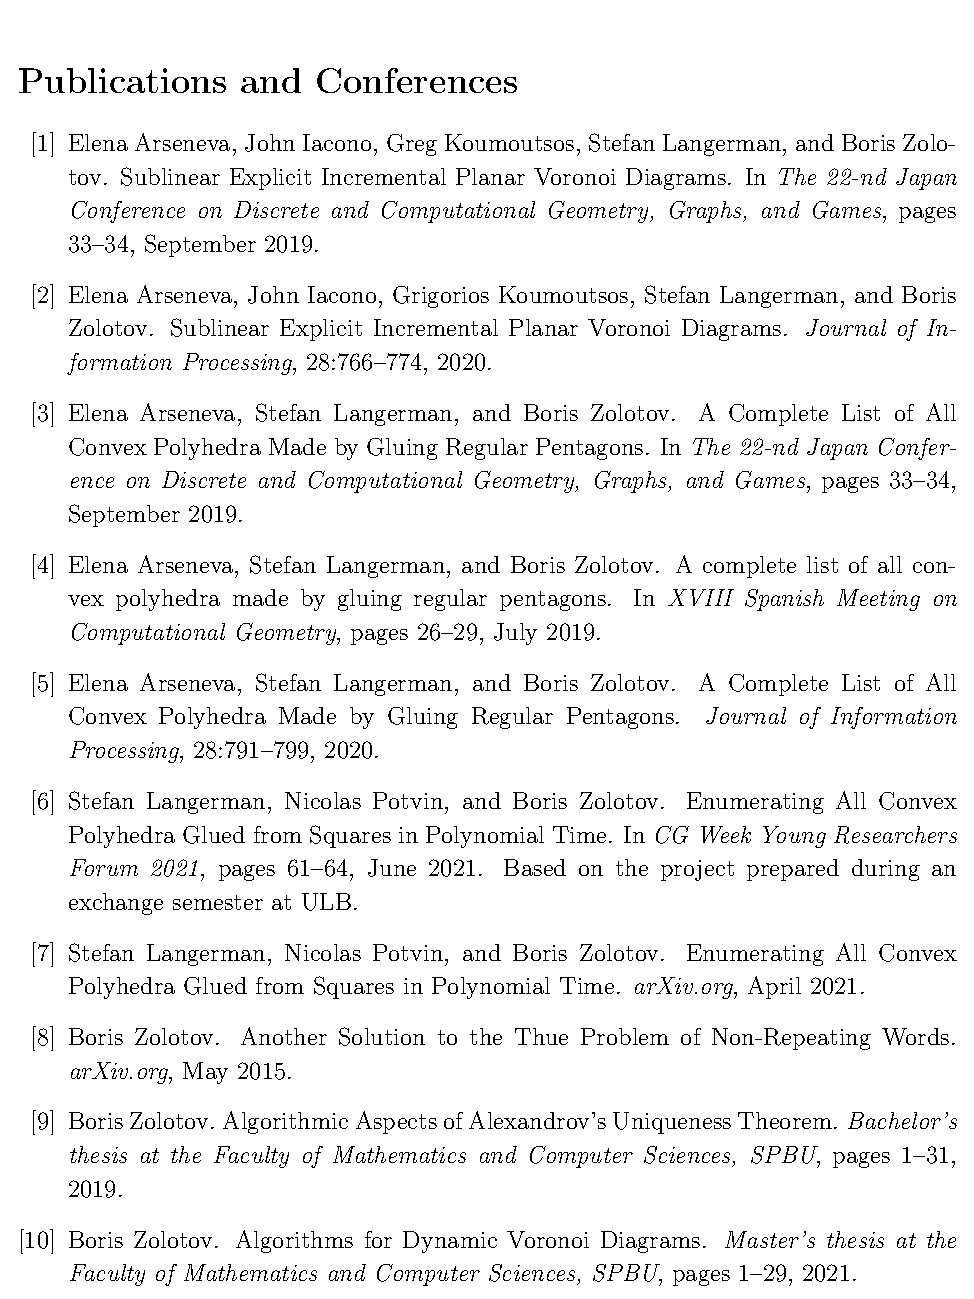
\includegraphics[width=0.97\textwidth]{boris-pub}
\end{center}

\end{document}
